% Compile with the XeLaTeX engine (on Overleaf: Menu -> Compiler -> XeLaTeX).
%\documentclass[11pt,a4paper]{article}
%\documentclass[a4paper,fleqn]{cas-sc}
%\documentclass[a4paper,fleqn]{cas-dc}
%\usepackage[authoryear]{natbib}
%\usepackage{fontspec}
%\setmainfont{Latin Modern Roman}
%\setsansfont{Latin Modern Sans}
%\setmonofont{Latin Modern Mono}
%\usepackage{fontspec}
%\setmainfont{DejaVu Serif}[Scale=0.92]
%\setmonofont{DejaVu Sans Mono}[Scale=0.82]
%\usepackage{polyglossia}
%\setmainlanguage{english}
%\setotherlanguage{russian}
%\usepackage[a4paper,margin=2.5cm]{geometry}
%\usepackage{amsmath,amssymb}
%\usepackage{booktabs}
%\usepackage[font=footnotesize,labelfont=bf]{caption}  % smaller font for figure/table captions
%\usepackage{tabularx}
%\newcolumntype{L}{>{\raggedright\arraybackslash}X}
%\usepackage{graphicx}
%\usepackage{microtype}
%\usepackage[numbers,sort&compress]{natbib}
%\usepackage[hidelinks]{hyperref}
%\usepackage{xurl}  % break long URLs across lines
% Layout settings: suppress overfull lines without loose justification.
%\graphicspath{{figures/}}
%\tolerance=1400
%\emergencystretch=2.5em
%\hbadness=2200
%\frenchspacing


%% 
%% Copyright 2019-2021 Elsevier Ltd
%% 
%% This file is part of the 'CAS Bundle'.
%% --------------------------------------
%% 
%% It may be distributed under the conditions of the LaTeX Project Public
%% License, either version 1.2 of this license or (at your option) any
%% later version.  The latest version of this license is in
%%    http://www.latex-project.org/lppl.txt
%% and version 1.2 or later is part of all distributions of LaTeX
%% version 1999/12/01 or later.
%% 
%% The list of all files belonging to the 'CAS Bundle' is
%% given in the file `manifest.txt'.
%% 
%% Template article for cas-sc documentclass for 
%% single column output.

\documentclass[a4paper,fleqn]{cas-sc}

% If the frontmatter runs over more than one page
% use the longmktitle option.

%\documentclass[a4paper,fleqn,longmktitle]{cas-sc}

% \usepackage[numbers]{natbib}
\usepackage[authoryear]{natbib}
% \usepackage[authoryear,longnamesfirst]{natbib}

\usepackage{subcaption}
\usepackage{tabularx}
\usepackage{graphicx}
\graphicspath{{figures/}}
\usepackage{xcolor, soul}
% cas-common.sty defines L as a non-wrapping fill column; the feature tables need a wrapping one.
\newcolumntype{L}{>{\raggedright\arraybackslash}X}

%%%Author macros
\def\tsc#1{\csdef{#1}{\textsc{\lowercase{#1}}\xspace}}
\tsc{WGM}
\tsc{QE}
%%%

% Uncomment and use as if needed
%\newtheorem{theorem}{Theorem}
%\newtheorem{lemma}[theorem]{Lemma}
%\newdefinition{rmk}{Remark}
%\newproof{pf}{Proof}
%\newproof{pot}{Proof of Theorem \ref{thm}}

\begin{document}
\let\WriteBookmarks\relax
\def\floatpagepagefraction{1}
\def\textpagefraction{.001}


\shorttitle{Integrated World Model}    

\title[mode = title]{An Integrated World Model for Strategic Planning and Scenario Analysis}
\author[1]{Nazar S.~Sotiriadi}
\cormark[1]
\ead{sotiriadi.n.s@gmail.com}
\author[1,2]{Andrei A. Osiptsov}[]
\affiliation[1]{organization={JSC Sberbank of Russia}, addressline={Kutuzovsky avenue, 32}, city={Moscow}, citysep={}, postcode = {121170}, country={Russian Federation}}
\affiliation[2]{organization={Skolkovo Institute of Science and Technology (Skoltech)}, addressline={Bolshoy Boulevard 30, bld. 1}, city={Moscow}, citysep={}, postcode = {121205}, country={Russian Federation}}

\date{\today}

%\begin{document}
\maketitle

\begin{abstract}
\noindent
Strategic planning requires tools integrating climate, economy, society, and geopolitics within a single framework, as sectoral models omit critical cross-domain feedbacks. We present a global integrated model (GIM) coupling 57 country agents with climate, carbon cycle, resource, socio-political, and financial dynamics in an annual loop. The economy uses a nested CES production function; climate follows an IPCC AR6 four-pool carbon cycle and two-layer energy-balance model; social tension, institutional legitimacy, and conflict risk respond to economic stress; crises (debt, currency, regime collapse) are threshold-triggered. Uncertainty is quantified via history-matched ensembles. Retrospective validation (2015--2023) yields RMSE of 0.60 trillion USD for GDP, 0.94 Gt for CO$_2$, and $0.145^{\circ}$C for temperature. A temporal hold-out (parameters constrained through 2019, evaluated on 2020--2023) gives out-of-sample errors of 0.77 trillion USD, 0.71 Gt, and $0.13^{\circ}$C respectively. The conflict-risk index achieves AUC 0.739 (bootstrap 95\% CI [0.60, 0.86], permutation $p\approx 0.001$). Ensemble uncertainty quantification at the ten-year horizon shows median world product of ${\sim}136$ trillion USD and a temperature anomaly of $1.1$--$2.0^{\circ}$C (5th--95th percentile). The model reveals cross-sectoral spillovers invisible to single-domain models: carbon taxes lower emissions but raise social tension; oil shocks propagate into sovereign debt crises; crop failures amplify protest pressure. A game-mechanical layer over the same core serves as a stress test, uncovering structural defects not visible in retrospective validation. GIM provides a coherent platform for scenario analysis, uncertainty quantification, and weak-signal detection, though it remains an exploration tool, not a forecast engine.

\medskip
\noindent\textbf{Keywords:} integrated assessment model, strategic planning, scenario analysis, uncertainty quantification, risk management, weak signals.
\end{abstract}


\section{Introduction}

Strategic planning and long-horizon scenario analysis require tools that treat climatic, economic, and socio-political processes jointly. Sectoral models address isolated domains: climate models describe atmospheric physics without finance or politics; integrated assessment models (DICE, RICE, FUND) couple economy and climate but lack sovereign finance, interstate relations, and social dynamics; macroeconomic models detail monetary flows but ignore natural capital. The mutual influence of these domains---warming to crop yields to prices to social tension to instability---falls outside any single model. This gap is substantive for strategic planning and systemic risk management, where the task is tracing shock propagation across interconnected subsystems and comparing alternative development trajectories.

This paper describes a model built to fill this gap. We emphasize from the outset: the model does not claim infallible prediction. Professional growth forecasts at two-to-five-year horizons often fail to beat naive extrapolation \citep{celasun2021}. A realistic goal is coherent scenario reproduction with proper uncertainty tracking, not point prediction.

The novelty lies in integration and coupling breadth: (i) a single annual loop carrying state through economy, climate, resources, society, politics, and interstate relations including discrete crises, where comparators stop at two or three domains; (ii) uncertainty quantification (ensembles, history matching) built into the workflow; (iii) an optional strategy layer where language-model agents set policies while consequences are computed deterministically. The crisis module and language-model layer are components of this integration.

Integrated assessment models (DICE, FUND) and large frameworks (GCAM, MESSAGEix, REMIND) couple economy and climate in detail but contain no sovereign finance, interstate relations, or socio-political dynamics; classic world-system models (World3) lack explicit price economy and modern climate. GIM's distinguishing feature is carrying the loop through society, geopolitics, discrete crises, and embedding language-model agents playing as countries (Table~\ref{tab:compare}, Section~\ref{sec:repo}). A controlled benchmark quantifying this advantage is in Appendix~\ref{app:benchmark}.

\begin{table*}[t]
\centering
\caption{Feature comparison with representative integrated, energy-economy, and world-system models. Each cell states specific capability; the last column lists domains outside each model's scope.}
\label{tab:compare}
\small
\begin{tabularx}{\linewidth}{@{}l L L l L@{}}
\toprule
Model & Paradigm & Domains covered & Spatial units & Not represented \\
\midrule
DICE\,/\,RICE & welfare optimisation & climate + aggregate economy, quadratic damages & world (RICE: 12 regions) & prices, finance, resources, society, politics, conflict, discrete crises \\
GCAM & recursive-dynamic market equilibrium & energy--land--water--climate detail & 32 regions & sovereign finance, social/political dynamics, interstate conflict \\
MESSAGEix & energy-system optimisation (+MACRO) & energy technology detail, land use, climate & 11+ regions & society, politics, geopolitics; crises as scenario inputs \\
E3ME & econometric simulation \citep{mercure2018} & energy--economy--environment, demand-led macro & $\sim$70 regions & interstate relations, conflict, endogenous discrete crises \\
T21\,/\,iSDG & system dynamics \citep{barney2002} & country-level economy--society--environment (SDG scope) & one country per model & interstate trade, geopolitics, multi-country shock propagation \\
World3 & system dynamics \citep{meadows1972} & global stocks: population, capital, resources, pollution & global aggregates & price economy, countries, modern climate, politics \\
GIM (this paper) & recursive simulation of interacting country agents & economy/prices, climate/carbon, resources, society/politics, geopolitics/conflict, crises, stock-flow-consistent finance & 57 country agents & sectoral energy technology detail, optimal-policy search \\
\bottomrule
\end{tabularx}
\end{table*}

The coverage comparison (Table~\ref{tab:compare}) is complemented by \emph{methodological axes}: listed models address different problems; direct ``better--worse'' ranking is inappropriate. In \emph{solution paradigm}, DICE/RICE/FUND and REMIND rest on welfare optimization; GCAM and MESSAGEix on detailed equilibrium; World3 on system dynamics of global aggregates; GIM is recursive simulation with adaptive expectations. Assessment models are \emph{deeper} within domains; GIM complements them. Its distinction appears along three dimensions: (i) breadth of coupling to society, geopolitics, discrete crises---quantified in Appendix~\ref{app:benchmark}; (ii) uncertainty as first-class object---ensembles and history matching built in; (iii) testability of non-standard blocks (conflict-risk AUC, identified lagged economy-society channel). GIM occupies the niche of broad scenario coverage and shock-propagation analysis.

\section{The model and its architecture}


\subsection{General design}

The model represents the world as 57 interacting countries evolving annually: the 50 largest economies (Taiwan included) plus seven residual regional aggregates conserving world totals. Each country's state comprises economic, resource, social, political, and military variables plus bilateral relations. Global evolution includes climate, carbon cycle, and world resource prices. One step is one year; blocks update in fixed order; outputs serve as inputs to subsequent blocks. The core is deterministic; uncertainty via ensembles with random parameter draws (Section~\ref{sec:calib}).

\subsection{Economy}

Each country's output is determined by capital, employed population, and energy. Production is a nested constant-elasticity-of-substitution function normalized to Cobb--Douglas at the calibration base point \citep{arrow1961}:
\begin{equation}
Y = A \, \Theta \, K^{\alpha} L^{\beta} E^{\gamma}, \quad \alpha = 0.30,\; \beta = 0.60,\; \gamma = 0.042,
\label{eq:prod}
\end{equation}
where $A$ is total factor productivity and $\Theta$ technology level. The nested form with capital--energy substitution elasticity $\sigma_{KE}=0.4$ \citep{vanderwerf2008,koetse2008} captures substitution difficulty: as energy becomes expensive, the economy shifts to capital and reduces energy use.

Equation~\eqref{eq:prod} is the Cobb--Douglas limit. The actual core is nested CES:
\begin{equation}
Y = A\,\Theta\,\Big[\mathrm{KE}_0\big(a_K (K/K_0)^{\rho} + a_E (E/E_0)^{\rho}\big)^{1/\rho}\Big]^{\alpha+\gamma} L^{\beta}, \quad \rho = \frac{\sigma_{KE}-1}{\sigma_{KE}},
\label{eq:ces}
\end{equation}
with weights $a_K = \alpha/(\alpha+\gamma)$, $a_E = \gamma/(\alpha+\gamma)$, base-point quantities $(K_0,E_0)$, and normalization $\mathrm{KE}_0 = K_0^{a_K} E_0^{a_E}$. At base point, bracket equals one, so \eqref{eq:ces} coincides with \eqref{eq:prod} in level and first derivatives for any $\sigma_{KE}$---normalized-CES discipline keeping calibration point invariant while substitution away is governed by $\sigma_{KE}=0.4$ (gross complementarity). Exponent sum $\alpha+\beta+\gamma = 0.942$ encodes mild decreasing returns (proxy for fixed factors); because each country carries a scale factor, renormalising to constant returns moves 2100 world product only 7--9\%.

This mechanism allows carbon price to restructure the economy. Capital accumulates by:
\begin{equation}
K_{t+1} = (1-\delta)\,K_t + s\,Y_t, \quad \delta = 0.05,
\label{eq:capital}
\end{equation}
with savings rate $s\approx0.24$ modulated by social stability and tension---precautionary saving \citep{mody2012}. Productivity $A$ grows at baseline ${\approx}1\%$/year, responding to R\&D spending, technology diffusion via trade, and conditional convergence (poorer economies catch up faster; slope 0.0093 per log unit of per-capita output gap to frontier, fit to 2015--2023 cross-section, reproducing China's and India's catch-up). Forward projections anchored to SSP2 \citep{riahi2017}. Energy, resource, and capital markets clear via prices with calibrated elasticities. Inflation (Phillips curve with energy cost pass-through), unemployment (Okun's law), central-bank rate (Taylor rule \citep{taylor1993}), government budget/debt, and trade flows are tracked. Inflation includes a weak quantity-theory term (pass-through $\lambda\approx0.027$ from cross-country panel). The economic block reproduces the last decade of history.

Technological change enters through four channels: baseline drift, R\&D-stock mechanism \`a la Jones \citep{jones1995}, technology diffusion via trade, and structural decarbonisation calibrated on 2015--2023 per-country decline. Endogenous renewable learning curves are not in the core---a simplification relative to energy-system models. Demography is exogenous in headline runs (logistic transition implemented but off by default); migration responds to income gaps and instability via gravity. No dedicated pandemic submodel; epidemic shocks are extreme events. Calibration sources: Penn World Table, World Development Indicators, SSP2 scenarios (IIASA database). Full dataset list in repository~\citep{theclimateguy2026gim}.

\subsection{Climate and the carbon cycle}

CO$_2$ emissions accompany output, with land-use source added. Emission intensity declines structurally at country-specific rates rising with development (fit to 2015--2023 per-country decline).

Carbon cycle uses IPCC AR6 four-pool impulse-response model \citep{joos2013}:
\begin{equation}
C^{(i)}_{t+1} = C^{(i)}_t e^{-1/\tau_i} + a_i E_t, \quad a = (0.217, 0.224, 0.282, 0.276), \quad \tau = (\infty, 394, 36.5, 4.3)\ \text{yr},
\label{eq:pools}
\end{equation}
so 21.7\% of each ton is permanent; rest decays on centennial, decadal, interannual scales. Radiative forcing $F = 5.35 \ln (C/C_0) + F_{\mathrm{non\text{-}CO_2}}$; non-CO$_2$ follows SSP2-4.5 marker pathway. Warming computed by two-reservoir surface--ocean heat-balance model \citep{geoffroy2013}:
\begin{equation}
C_s \dot T = F - \lambda T - \kappa\,(T - T_d), \quad C_d \dot T_d = \kappa\,(T - T_d),
\label{eq:ebm}
\end{equation}
with feedback $\lambda$ set by equilibrium climate sensitivity, heat capacities and exchange coefficient calibrated to \citet{geoffroy2013}. This is reduced-complexity emulator architecture (FaIR, MAGICC; \citealp{smith2018fair,meinshausen2011}). Block passes: equilibrium climate sensitivity $3.0^{\circ}$C (AR6 best estimate), transient climate response $1.79^{\circ}$C under 1\%/year CO$_2$ ramp (AR6 best estimate 1.8, likely range 1.4--2.2).

Tipping points and carbon feedbacks: proportional temperature-dependent flux and stochastic abrupt-release channel (heavy-tailed) are switchable and \emph{off} in headline runs---deeply uncertain, not validated. Explored in tail-risk scenarios. Block calibrated to IPCC AR6 WG1, Global Carbon Budget \citep{friedlingstein2023}: driven by observed emissions from pre-industrial spin-up, tracks 1990--2023 temperature with error $0.096^{\circ}$ C and best-fit ECS $3.0^{\circ}$C.

\subsection{Warming damages and the cost of carbon}

Warming reduces output via quadratic damage function \citep{nordhaus2017,howard2017}:
\begin{equation}
\Omega(T) = 1 - 0.0078\,T^{2},
\label{eq:damage}
\end{equation}
giving losses 3.1\%, 7.0\%, 12.5\% at +2, +3, $+4^{\circ}$C. Coefficient anchored to Howard--Sterner meta-analysis central estimate (${\approx}7\%$ at $+3^{\circ}$C)---roughly three times DICE-2016R2. Damage multiplier normalised to 2023 baseline. A Burke-type growth-damage channel (temperature-dependent productivity growth increment) is switchable and off by default (contested mechanism). Social cost of carbon computed by marginal-pulse method; depends on discounting and growth structure. Results in Section~\ref{sec:calib}. Sources: Howard--Sterner, Burke et al., EPA-2023, RFF-SP.

\subsection{Resources}

For each country, stocks, production, consumption of energy, food, metals tracked; world prices rise when demand exceeds supply, passed into inflation and economy. Resource market clears by price with calibrated demand elasticity; slow-adjustment fallback. Resources in aggregate, not detailed sectoral energy systems. Sources: World Development Indicators; price elasticities from generalized market estimates.

\subsection{Society, politics, geopolitics, and culture}

For each country, trust in government, social tension, income inequality, institutional legitimacy, protest pressure tracked. These respond to economy---rising inflation/unemployment raise tension, erode trust; inequality amplifies. Bilateral relations: trade volume, alliance, conflict/tension, war, sanctions. Military capability anchored to CINC-style composite (population, energy, GDP, SIPRI military expenditure). Military-expenditure component matters empirically: three-component proxy correlates with levels ($\approx 0.76$) but anti-correlates with post-2022 militarization dynamics (-0.115). Cultural traits (individualism, uncertainty avoidance, long-term orientation, hierarchy) and regime type influence behavior \citep{hofstede2010}. Socio-political priors tied to literature where possible; remainder expert-set (Section~\ref{sec:uq}). Sources: SWIID, World Bank Gini, Worldwide Governance Indicators, UCDP/PRIO Armed Conflict Dataset, Correlates of War CINC, SIPRI military expenditure, Global Sanctions Database, Hofstede indices. Traits not affecting outcomes removed.

Social tension operational definition: latent index on [0,1] constructed as fixed-weight composite of observed quantities at base year: $0.35(1-\text{trust}) + 0.25\,\text{Gini(norm)} + 0.15\,\text{water stress} + 0.10\,\text{climate risk} + 0.15(1-\text{regime stability})$, rescaled WGI to [0,1]. Evolves by increments: unemployment adds 0.010/point, inflation 0.005/point, inequality proportional to Gini damped by individualism, mean-reversion to trust anchor, long-term orientation damps total, small spillover (0.05) from neighbours. Coefficients varied in ensembles (Appendix~\ref{app:params}).

Institutions endogenous: legitimacy = $0.6\,\text{trust} + 0.4(1-\text{tension})$; with protest pressure and debt stress determines policy space multiplier; crises knock regime stability. Regime type (democracy/autocracy/hybrid) fixed categorical; modulates responses. Regime collapse resets state variables but not type. State-dominated economies represented by same forms with country-specific states; state-owned credit, administered prices not structurally modelled (limitation, Section~\ref{sec:limits}).

\subsection{Risk, crises, and finance}

Discrete crises---debt, currency, regime collapse, extreme climate---triggered when thresholds crossed. Severity heavy-tailed (optional). Financial side: strict accounting; government finances closed; private sector full bank balance sheet; every loan creates matching deposit; money stock identically deposits/loans; excessive borrowing raises credit cost---financial accelerator \citep{bernanke1999,godley2007}. Each country runs independent central bank: policy rate follows Taylor rule, capped $\pm{}$ 6 pp around neutral. Nominal exchange rates not modelled (common real numeraire); currency crisis triggered by fundamentals: external debt >50\% GDP, current-account deficit >4\%, reserves <3 months imports. Sovereign distress: debt crisis fires when debt >120\% GDP and effective rate (policy + sovereign spread) >12\%; crisis applies 40\% write-down, 7\% output loss; unresolved decays further; exit requires debt <70\% GDP, rate <8\%, within 6 years. International capital flows represented at needed level: bilateral trade settles in reserves; net exports sum to zero; reserve depletion feeds currency trigger. Full portfolio capital account not modelled (limitation).

\subsection{Block interactions}

Connectivity is key: economy emits; emissions warm; warming damages output; carbon price raises energy cost, reduces emissions. Economic hardship raises tension, lowers trust, changes savings rate, raises crisis risk; crises hit output/capital, transmit to trading partners. Resource scarcity raises prices/inflation; conflicts/sanctions disrupt trade. Bilateral flows settled in reserves; net exports tracked explicitly; world sums to zero; persistent deficits drain reserves, raise external debt, feed currency trigger. Bilateral trade follows gravity law (distance elasticity ${\approx}0.9$; \citealp{headmayer2014}); conflict, unrest, climate risk spill over to neighbours. Geographic coupling leaves 2015--2023 retrospective fit essentially unchanged (world product, CO${}_2$, temperature RMSE move <0.25\%).

\begin{figure}[t]
\centering
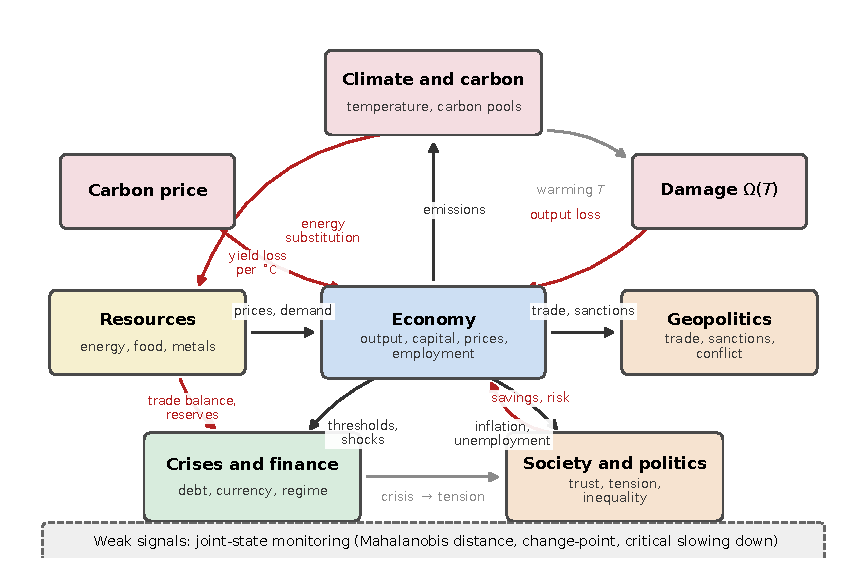
\includegraphics[width=\linewidth]{fig1_architecture.pdf}
\caption{Model architecture and links between blocks. Economy central hub; black arrows direct effects, red arrows feedbacks reducing output/savings. Closed climate loop (emissions\ensuremath{\to}warming\ensuremath{\to}damage\ensuremath{\to}output) complemented by carbon-price, resource, socio-political, geopolitical, and discrete-crisis blocks. Bottom layer: continuous monitoring for weak signals.}
\label{fig:arch}
\end{figure}

\section{Calibration and validation}
\label{sec:calib}


\subsection{Data sources}

Each block anchored to external data (Table~\ref{tab:data}). Economic and climate blocks calibrated and validated most rigorously; socio-political/geopolitical variables anchored to recognized indices, assessed against softer criterion.

\begin{table*}[t]
\centering
\caption{Empirical basis of model blocks.}
\label{tab:data}
\small
\begin{tabularx}{\linewidth}{@{}l L L@{}}
\toprule
Block & Data source & Purpose \\
\midrule
Economy & Penn World Table, World Development Indicators & factor shares, growth, debt \\
Climate and carbon & IPCC AR6 assessment, Global Carbon Budget & sensitivity, $T$, CO${}_2$ paths \\
Cost of carbon & EPA-2023, RFF-SP & reference cross-check \\
Forward growth & SSP2 scenarios & forward productivity drift \\
Conflict & UCDP Georeferenced Event Dataset & conflict-risk validation \\
Inequality & SWIID & income inequality \\
Institutions & Worldwide Governance Indicators & legitimacy, governance quality \\
Military power & CINC-style composite incl.\ SIPRI military expenditure & country capability \\
Culture & Hofstede indices & cultural traits \\
\bottomrule
\end{tabularx}
\end{table*}

\subsection{Calibration principles and integrity control}

Calibration rules: (1) optional mechanisms switchable, off by default unless anchored by evidence; (2) parameter estimation uses history matching not point fitting: discard parameter regions incompatible with observations, leaving not-yet-ruled-out (NROY) region \citep{williamson2013}. Constraining observations: 2015--2023 retrospective series of world product, emissions, temperature. For candidate $\theta$, implausibility $I_o(\theta) = \mathrm{RMSE}_o(\theta) / \mathrm{tol}_o$; tolerances (6 trillion USD, 2 Gt, $0.15^{\circ}$ C) bundle observational uncertainty and model-discrepancy; retain if $\max_o I_o \le 3$ (3-sigma). Core deterministic, one simulation per vector; when internal variability on, evaluated over 8-seed mini-ensemble. Exterior cross-checks (SCC range, conflict ranking) as additional constraints. (3) climate coefficients from initial state tightly bound to input data checksum; integrity checked automatically. (4) regression control: key retrospective-validation quantities pinned; changes must preserve or recalibrate.

Temporal hold-out: history matching using data through 2019; NROY region frozen; 2020--2023 segment scored out-of-sample (at 3-sigma cut, 2015--2019 window retains full prior region---60 draws none ruled out---so frozen region coincides with prior box; test conservative). Out-of-sample errors reported alongside in-sample (Table~\ref{tab:backtest}). Held-out segment contains COVID-19; skill reported raw and with 2020 excluded. Reproducible harness: \texttt{scripts/run\_holdout\_validation.py}.

Crisis thresholds: debt crisis at debt >120\% GDP, effective rate >12\%; currency crisis at external debt >50\% GDP, current-account deficit >4\%, reserves <3 months imports; regime collapse at trust <0.20, tension >0.80. These are expert priors informed by Maastricht, Reinhart-Rogoff, first-generation currency-crisis models, tagged \texttt{PRIOR}; severity/persistence multipliers calibrated to retrospective plateau. Registry auditable parameter by parameter.

\subsection{Resulting metrics}

Validation summary across blocks in Table~\ref{tab:backtest}. In-sample retrospective fit 2015--2023: RMSE GDP 0.60 trillion USD, CO${}_2$ 0.94 Gt, temperature $0.145^{\circ}$C (with internal variability spread re-derived from observed 1990--2023 forced residuals, $\sigma=0.088$, near-white). Temporal hold-out (constraints through 2019, evaluation 2020--2023): out-of-sample errors GDP 0.77 trillion USD, CO${}_2$ 0.71 Gt, temperature $0.13^{\circ}$C; with 2020 excluded: 0.83, 0.10, 0.15 respectively. Skill on held-out: temperature beats persistence (+0.05) and linear extrapolation (+0.16); emissions beats both (+0.32, +0.54); product loses to persistence (-0.42) and linear trend. Hold-out confirms in-sample fit not artefact.

Comparison with benchmark forecasts: model beats persistence for temperature (skill +0.14) and marginally for product; loses to linear extrapolation for product and emissions over short smooth interval---expected \citep{celasun2021}.

Without SSP2 anchor: emergent no-intervention baseline lands near strong-mitigation end (${\approx}2^{\circ}$C by 2100, closest SSP1-2.6): structural decarbonisation rate from 2015--2023 optimistic extrapolated decades. Recommended use: scenario differences, where anchor uncertainty cancels.

Conflict block: conflict-proneness score fixed-weight composite of observed inputs---$0.35(1-\text{regime stability}) + 0.25\,\text{social tension} + 0.20\,\text{climate risk} + 0.20\,\text{military burden}$---no coefficient estimated from conflict data; weights fixed at design. Each input enters at its base-year 2023 value from the committed grounding files. Compared with UCDP/PRIO armed conflicts 1990--2023 across 57 countries \citep{sundberg2013}. AUC 0.739 (bootstrap 95\% CI [0.60, 0.86], 20,000 resamples \citep{efron1993}); permutation $p\approx0.001$. Vintage-clean configuration (inputs from pre-2000 data only, evaluated against 2000--2023 conflicts, 49 direct countries) yields AUC 0.84 (bootstrap [0.72, 0.94], $p\approx4\times10^{-5}$)---identical to the 2023-vintage score evaluated on the same subset and window---so the ranking skill is not an artefact of post-conflict input contamination (conflict itself degrades regime stability and raises the military burden). Reproducible harness: \texttt{scripts/run\_conflict\_vintage\_test.py}. Brier skill relative to base-rate +0.123. Split into quintiles: observed conflict incidence falls monotonically from 55\% top to 8\% bottom. Score modest but appropriate comparison class is conflict forecasting.

Social cost of carbon: under modern Ramsey scheme with near-zero pure time preference ${\approx}\$90$/tCO$_2$ at a 200-year horizon (below EPA-2023/RFF-SP ${\approx}\$190$); under Nordhaus discounting ${\approx}\$22$, \$43, \$46 at 30-, 100-, 200-year horizons. Across calibrations, SCC varies \$90--280/tCO${}_2$. Fed DICE-2016R2's lower damage coefficient, pulse engine returns ${\approx}\$15$---below DICE's \$31---so DICE underestimates damages relative to our function. SCC sensitivity dominated by $(\rho,\eta)$ choice interacting with growth path. Values are reported at the 200-year horizon, where the integral has converged (extending to 300 years moves the DICE-damage benchmark by about $1\%$); the 30-year figure shows what horizon truncation alone removes.

\begin{table*}[t]
\centering
\caption{Validation summary by model block: data source, validation criterion, achieved result. Economic and climate blocks checked by retrospective evaluation (in-sample and temporal hold-out). Others: softer criterion---cross-check, benchmark improvement, or channel identification.}
\label{tab:backtest}
\small
\begin{tabularx}{\linewidth}{@{}l l L L@{}}
\toprule
Block & Source & Criterion & Result \\
\midrule
Economy & PWT, WDI & in-sample RMSE 2015--2023; hold-out 2020--2023 & GDP \$0.60T in-sample; \$0.77 out-of-sample \\
Climate and carbon & IPCC AR6, GCB & in-sample RMSE 2015--2023; hold-out 2020--2023; ECS/TCR anchors & CO${}_2$ 0.94 Gt in-sample, 0.71 out-of-sample; T $0.145^{\circ}$C in-sample, 0.13 out-of-sample \\
Cost of carbon & EPA-2023, RFF-SP & published cross-check; Ramsey discounting & ${\approx}\$90$/tCO$_2$ (range 90--280); under DICE damages ${\approx}\$15$ \\
Conflict & UCDP/PRIO & ranking vs.\ registry & AUC 0.739 [0.60; 0.86]; BSS +0.123; $p\approx 0.001$ \\
Social block & SWIID, WGI & channel identification (Sec.~\ref{sec:uq}) & significant lagged channel; $p<10^{-12}$ \\
\bottomrule
\end{tabularx}
\end{table*}

\begin{figure}[t]
\centering
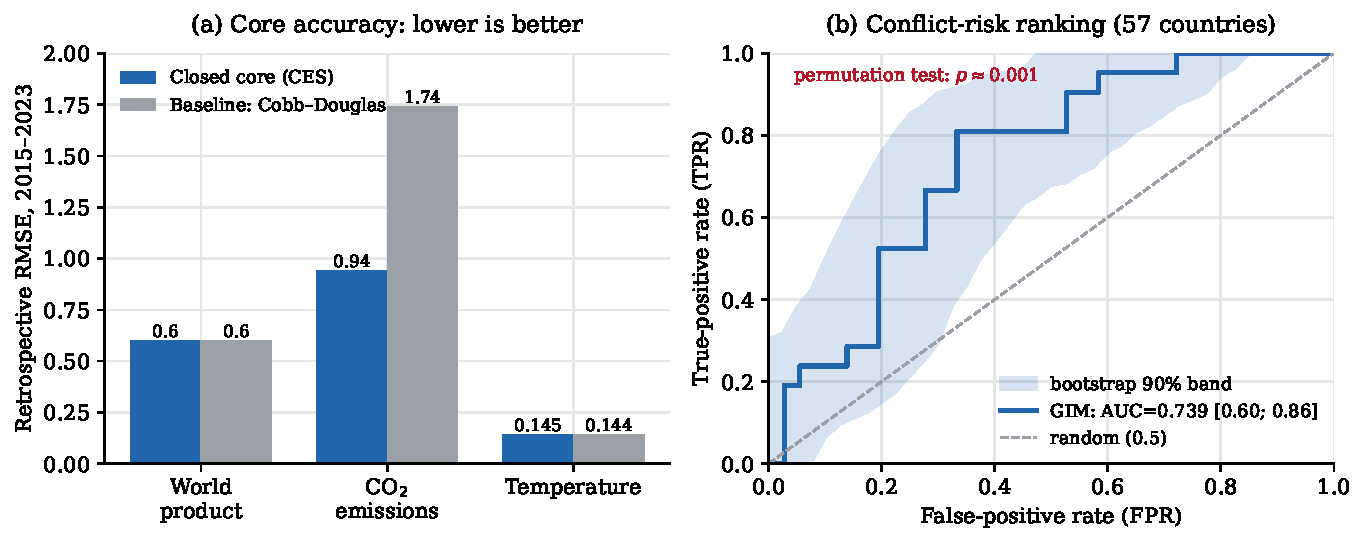
\includegraphics[width=\linewidth]{fig2_validation.pdf}
\caption{Retrospective validation. (a) RMSE 2015--2023 for nested CES vs former Cobb-Douglas core. (b) ROC curve conflict block (score inputs at 2023 base-year values; vintage-clean variant in text): AUC 0.739 (bootstrap 90\% band shaded; 95\% CI [0.60,0.86]; $p\approx 0.001$) vs 0.5 random.}
\label{fig:valid}
\end{figure}

\section{Uncertainty, sensitivity, and parameter identification}
\label{sec:uq}

Key question: parameters identified by data rather than hand-set. Each key parameter equipped with prior distribution---central value, plausibility range, literature source (Appendix~\ref{app:params}); estimation by history matching (Section~\ref{sec:calib}). $\sigma_{KE}=0.4$ rests on 0.3--0.5 estimates; $\delta=0.05$ on PWT 3--8\%; damage coefficient 0.0078 within empirical range 0.0015--0.025 at Howard-Sterner central.

Sensitivity analysis: global screening by Morris elementary-effects \citep{morris1991,campolongo2007} over 33 key parameters, 4 outputs (Fig.~\ref{fig:sens}; 8 trajectories, 10-year horizon). Temperature determined almost exclusively by climate parameters; world product by capital depreciation, energy intensity, damage coefficient; world emissions by emissions scale, land-use source, capital stock. Robust to screening budget: increasing trajectories $8\rightarrow 32$, Spearman $\rho\approx0.99$ for physical quantities; dominant parameters reappear. Social tension: $\mu^*$ three orders lower (noise floor); ranking unstable ($\rho\approx0.93$ $8\rightarrow 32$ vs. physical $\approx 0.99$). This does not mean society decoupled from economy: screening varies physico-economic priors only; tension governed by own parameters and responds to economic conditions with lag (Fig.~\ref{fig:social}). Morris complemented by Sobol-Saltelli over twenty most influential priors: output variance attributable (ECS dominates temperature, catch-up convergence dominates product, sovereign-spread coefficients dominate inequality); ten lower-ranked priors can be frozen---effective dimensionality far smaller.

Sobol--Saltelli total-order shares: ECS accounts for 0.95 of temperature variance (first-order 0.94); catch-up convergence 0.88 of product; the carbon-feedback coefficient 0.81 of CO$_2$ (live in this analysis, whose prior set excludes the artifact-bound emissions-scale and land-use terms); sovereign-spread curvature 0.86 of end-period inequality; ten lower-ranked priors fall below 0.01 on every output.

Ensemble uncertainty quantification: Monte Carlo ensemble (500 members) with random parameter draws. Result not single trajectory but distribution (Fig.~\ref{fig:ens}). World product denotes aggregate gross product of 57 modeled actors---50 largest economies (Taiwan included) plus 7 regional aggregates; 2023 base ${\approx}107$T. Cut at 50: direct countries carry ${\approx}93.5\%$ of world product; smallest ${\approx}0.25\%$---individually negligible; 57 actors keep full bilateral matrix cheap. 10-year median ${\approx}136$T, IQR ${\approx}134$--$139$, 5--95th ${\approx}131$--$142$; temperature anomaly 5--95th ${\approx}1.1$--$2.0^{\circ}$C. Reported percentiles converged: $80\to500$ members, median moves 0.5T (${\approx}0.4\%$), upper percentiles less; temperature median $0.05^{\circ}$C; lower tail tightens ${\approx}1.05\!\to\!1.1^{\circ}$C. Priors drawn independently cross-parameter correlations not imposed, slightly overstates spread---conservative direction. Convergence diagnosed empirically; percentile stability reported.

\begin{figure}[t]
\centering
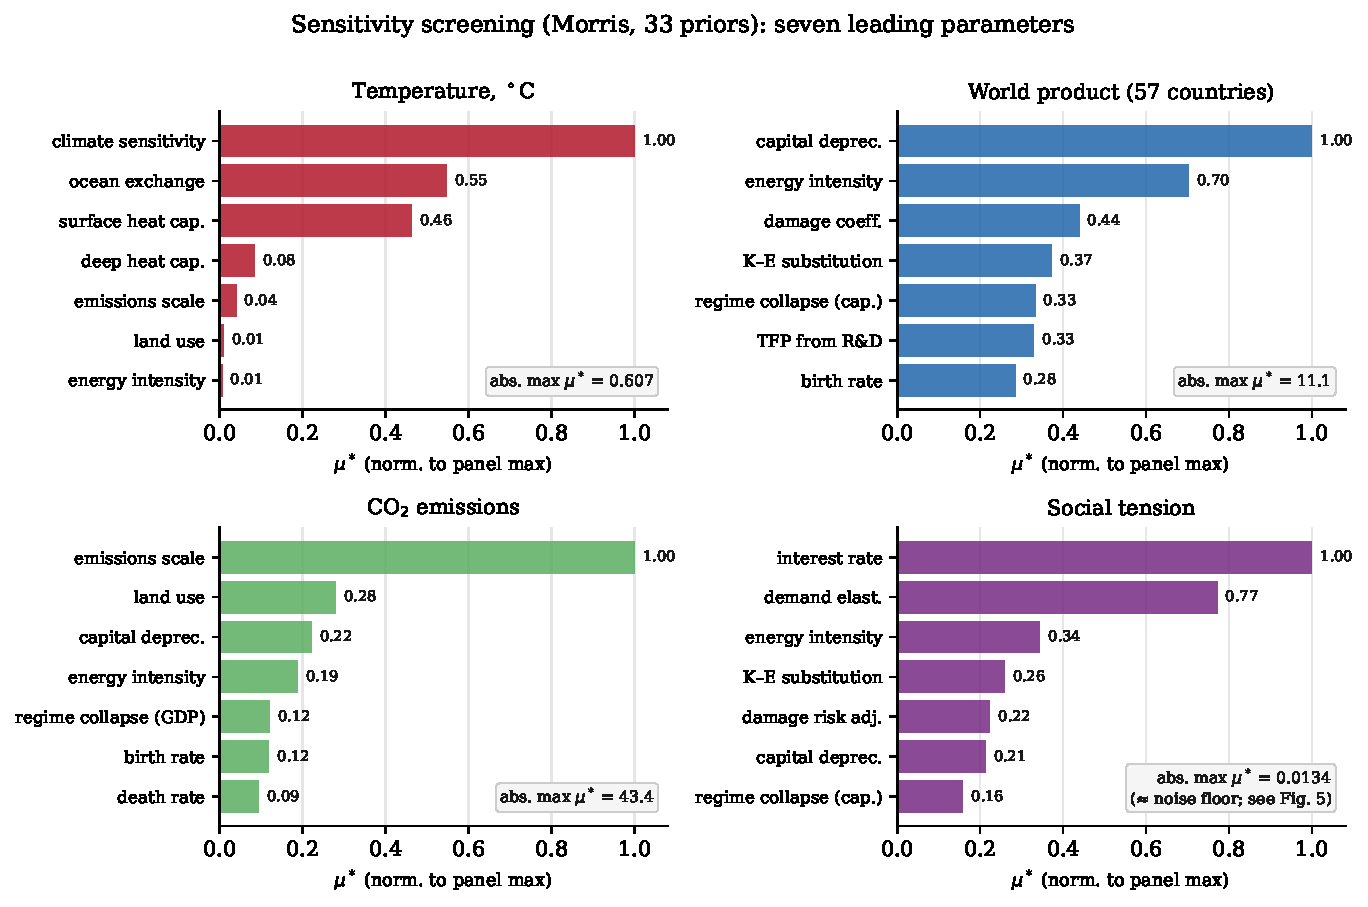
\includegraphics[width=\linewidth]{fig3_sensitivity.pdf}
\caption{Global sensitivity screening (Morris) over 33 parameters for 4 outputs (57 countries); 7 most influential shown, $\mu^*$ normalized to max within panel. Temperature governed by climate parameters; product and emissions by economic/emission parameters. Social tension $\mu^*$ three orders lower (noise floor); its channel examined in Fig.~\ref{fig:social}.}
\label{fig:sens}
\end{figure}

\begin{figure}[t]
\centering
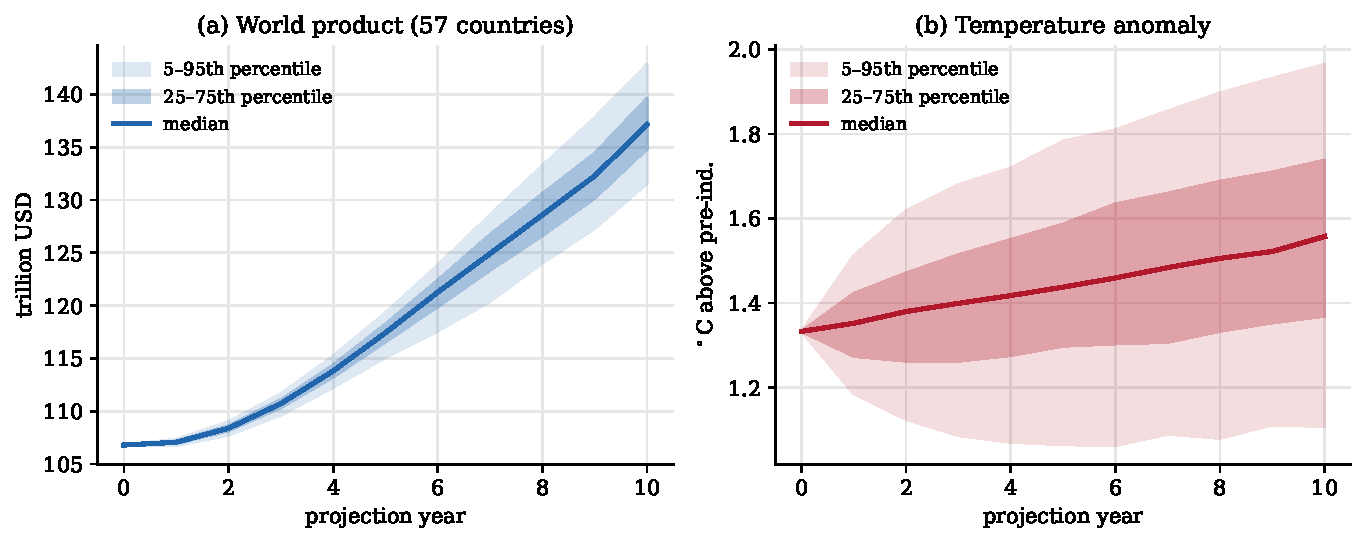
\includegraphics[width=\linewidth]{fig4_ensemble.pdf}
\caption{Ensemble uncertainty (500 members): Monte Carlo with random parameter draws. Median, 25--75th, 5--95th bands for (a) aggregate product of 57 countries and (b) temperature anomaly.}
\label{fig:ens}
\end{figure}

Channel from economy to social tension: low sensitivity of tension to physico-economic priors does not mean decoupling; tension accumulates (increment from unemployment, inflation, inequality), manifests with lag. Three checks (Fig.~\ref{fig:social}; reproducible in Section~\ref{sec:repo}). (1) Localization: ensemble varying social-block priors shows final tension governed by them---sensitivity to inequality (Spearman $\rho\approx+0.59$, $p<10^{-11}$), trust anchor ($\rho\approx-0.52$, $p<10^{-9}$)---physico-economic weak. (2) Accumulation: prior-induced spread grows with horizon (std dev increases ${\approx}2/3$ from 5 to 25 years)---lag signature. (3) Impulse response: exogenous stagflation shock raises mean tension persistently; response still building decade later (positive 78\% runs). Distributed-lag regression confirms significant contemporaneous transmission (lag 0: $p<10^{-8}$), positive cumulative effect over 5 lags. Channel significant but mediated and lagged.

Military-capability identification: 48-country panel military expenditure 1995--2024 (country fixed effects, clustered errors): peacetime spending growth tracks output growth nearly one-for-one (coefficient 0.79, $p<0.001$); post-2022 excess structured by geography---NATO frontier states $+13$ pp/year, others ${\approx}0$; Richardson action-reaction rejected ($p=0.74$). Motivates grounding: military expenditure as observed state variable, not autonomous arms-race; threat-dependent shift carried by dyadic relations.

Computational cost: single consumer laptop (Apple M4 Pro, 12 cores, 24 GB): one 57-actor world-year 30--50 ms; 10-year deterministic <1s; 500-member 10-year ensemble ${\approx}47$\,s across cores; Morris screening 2--3 min per output; Sobol--Saltelli (2,816 deterministic 2015--2050 runs) ${\approx}30$ min; full test suite ${\approx}2$ min. No cluster required; ensemble-first uncertainty practical.

\begin{figure}[t]
\centering
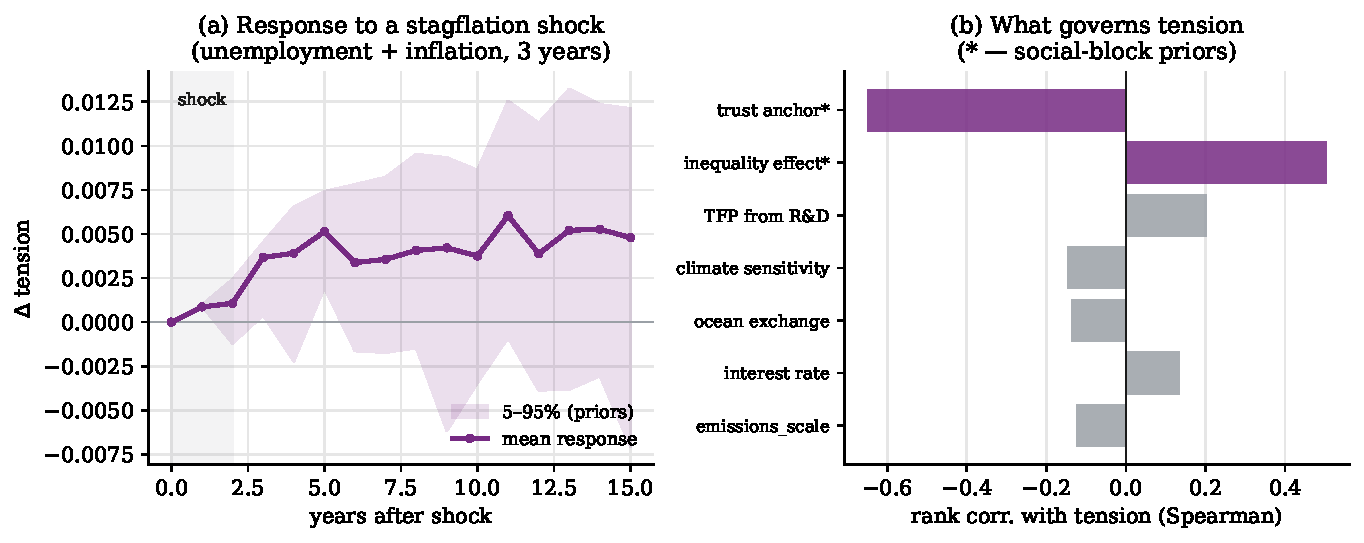
\includegraphics[width=\linewidth]{fig5_social_channel.pdf}
\caption{Influence of economic conditions on social tension. (a) Impulse response of mean tension to exogenous stagflation shock (unemployment and inflation, 3 years): mean curve and 5--95th band; response builds slowly, persists beyond decade. (b) Localization: rank correlation of priors with final tension; social-block parameters (marked *) dominate, not physico-economic.}
\label{fig:social}
\end{figure}

\section{Limitations}
\label{sec:limits}

Honest list of what model cannot yet do.

Expectations in headline run are adaptive; households/firms look to recent past, not rational anticipation. Model-consistent expectations implemented but marginal effect unstable; off by default.

Long-run growth weakly identified; endogenous R\&D-stock mechanism only weakly pinned by short history; forward projections anchored to external scenario.

Climate fast approximation, not full Earth-system; strongest carbon feedbacks deeply uncertain, relegated to tail scenarios.

Damage estimates uncertain across discipline; carried as interval, not single number.

Socio-political links partly anchored, partly expert. No single calibration dataset for discontent transition; substantial part of social-block priors tied to literature (war-size power-law tail, migration-gravity elasticities, regime-collapse GDP loss, conflict-onset forecast skill, geographic coupling against real spatial dependence). Expert-set: coupling thresholds, cross-border tension diffusion weight (no clean adjacency anchor; pure-adjacency protest spillover statistically insignificant in careful cross-national study). Economy-tension channel significant, directionally correct, lagged (Fig.~\ref{fig:social}); conflict intrinsically hard to predict; geopolitical block suitable only for relative risk (AUC ${\approx}0.74$; vintage-clean test bounds reverse causation).

Crisis triggers threshold-based; capture qualitative behavior without single fitted dataset; severity anchored to power-law of war sizes (exponent $\alpha\approx1.5$; Richardson, Clauset).

Geographic coupling realistic but payoff concentrated in trade channel (anchored gravity); cross-border diffusion weights for conflict, tension, climate risk modest; tension lacks clean literature anchor.

Overall stance unchanged: realistic goal calibrated against own uncertainty, not infallible foresight. Accuracy bar: improvement over naive benchmark.

\section{Typical use cases}
\label{sec:scenarios}

Model intended for three interrelated modes.

Scenario analysis and strategic planning: principal mode---comparison of baseline with perturbation/policy scenario (carbon price, resource scarcity, escalation) tracing propagation through economy, climate, society, geopolitics. Relative quantities matter, not absolute point values.

Worked policy case: \$50/tCO${}_2$ carbon tax. Against baseline, tax lowers emissions ${\approx}5.5\%$ over 10 years (first-order effect) while raising social tension and lowering trust via energy-price-inflation channel---political sustainability cost invisible to single-domain models, monotone in tax rate, directly relevant (French 2018, Australian 2014 reversals). Full dose-response in Appendix~\ref{app:benchmark}; run as ensembles; weak-signal profile comparison is intended early-warning reading.

Ensemble computations: uncertainty introduced by large ensembles with random parameter draws; yields distribution of outcomes; scenarios best compared as ensembles.

Weak-signal detection: complements threshold-based crisis logic. Three tools: Mahalanobis distance of joint state from baseline distribution \citep{mahalanobis1936,wilson1931}; structural-break detection via change-point with information-criterion penalty \citep{schwarz1978}; critical-slowing-down indicators (rising autocorrelation, variance) approaching bifurcation \citep{scheffer2009}. Series first reduced to stationary increments. On synthetic/model trajectories: injected 15\% product drop detected exactly; calm run near false-alarm rate. Working device: relative comparison of scenario's weak-signal profile with baseline's.

\section{Software implementation and the scenario environment}
\label{sec:repo}

Model implemented as open codebase, available at~\citep{theclimateguy2026gim}. Results correspond to release v18.1.3. Core deterministic and reproducible: each run written to dated folder with manifest; unit tests and validation protocol pin key quantities. Calibration datasets immutable, checksum-bound. Baseline, scenario questions, multi-agent games, calibration via single command-line; engine packaged as pip-installable library with runtime data.

Large language models as countries: country policy may be set by LLM agent. Agent receives observed state, returns coherent strategy compiled into formalized actions. Supported modes: rule, growth target, language model, precompiled doctrine; user sets update depth. Generative model produces intentions/strategy; consequences computed by deterministic empirically anchored core. This separation preserves reproducibility. Protocol: default backend DeepSeek-chat (temperature 0.4); any OpenAI-compatible endpoint or local Ollama substitutable. State serialized to JSON payload, embedded in fixed prompt with action schema; reply parsed as JSON, clamped to bounds; parsing/validation failure falls back to built-in rule---invalid actions never enter simulation. LLM agents off in all validated configurations; headline numbers involve no LLM. Multi-agent episodes archive prompts/responses for audit.

Hybrid games and "what-if" hypotheses: human and agent joint play. Action mode commits move; what-if mode plays hypothesis in isolation. Each move unfolds into ensemble, not single trajectory.

Interactive analytical environment: native desktop application over same deterministic engine. Natural-language assistant maps scenarios to levers; expert mode direct control; run-comparison against baseline; live validation panel. Every result from engine, never LLM; charts show command-line invocation. Exports: summary dashboard, analytical brief, logs.

Scenario environment operationalizes model purpose. Coupled core becomes platform for exercising multi-agent interaction; generative AI expands plausible strategies without supplanting empirically anchored mechanics.

\section{A game-mechanical simulation on the model core}
\label{sec:game}

Scenario environment extended to complete decision game (working title GODMODE, \url{https://godmode-rwhp.onrender.com/}): single player steers world 2023--2050 through ${\sim}30$ annual turns. Each year decision card presents dilemma from deck of 158 situations (109 shocks, 49 opportunities); chosen option compiled into typed policy actions; full 57-actor engine steps; consequences (output, prices, tension, trust, crises, wars) are engine's, not scripted. Run lost when any of seven catastrophe thresholds crossed (temperature, biosphere, stability, economic/geopolitical strain, energy/food prices); reaching 2050 with all gates intact wins. Game adds presentation/pacing; every consequence computed by deterministic core; one engine year 30--50 ms; full game ${\approx}1$\,s---large-scale balance testing statistically meaningful.

Report game for two reasons: outcome distributions are stress test under adversarial policy sequences; balancing uncovered structural properties---including two genuine defects---not surfaced by backtests or ensembles.

Outcome distributions: automated playthroughs by scripted policy archetypes: green (decarbonising), growth (expansionary), mixed (uniform random), passive (first option). Reference batch 1,002 games (334 per archetype, deterministic seeds; Fig.~\ref{fig:game}); overall survival 23.5\%, intended difficulty (one win in 4--6 attempts). Losses spread: 35\% climate, 22\% economic strain, 21\% geopolitical strain, 13\% social stability, 8\% energy price---no single dominant failure (tuned property). Failures cluster 2040--2045: 77\% losing games fail near finish (slow accumulators: temperature, debt, tension).

Emergent regularities robust across batches; properties of underlying model, not card deck. (1) No doctrinaire strategy dominates: mixed survives most (28.4\%), beating green (20.1\%) and growth (21.9\%); each dies of characteristic disease---green economic strain (43\% losses), growth climate and social stability (39\%, 34\%). Single-axis optimisation shifts binding constraint---game-mechanical face of coupling. (2) Passivity worst: always-first wins 18.7\%; dies overwhelmingly of economic strain (67\%). (3) Restraint on strain axes dominates single lever: prudent on economic and geopolitical strain wins ${\approx}75\%$; reckless on both ${\approx}5\%$. (4) Assistance mechanics moral-hazard cost: regional stabilization package lowers final win rate when underlying driver unaddressed.

Game layer not validation substitute; does not provide quantitative goodness-of-fit against historical data. Diagnostic value: exploring regions smooth historical trajectories don't visit; defects found there are genuine weaknesses.

Game as diagnostic instrument: balancing produced two model fixes. Play showed resource prices drifted to clamps; traced to missing equilibrium term in price rule and two quantity-side defects (frozen food-demand base, compounding recycling term)---fixed v18.1.2. Hawk-dove experiments showed government trust declining on indistinguishable paths---structural attractor from inequality drag ${\approx}40{\times}$ stronger than the only positive trust term; fix (opt-in equilibrium anchor, v18.1.3) lifted floor, removed spurious oscillation. Neither defect visible in 2015--2023 backtests---both live in corners only long adversarial trajectories visit. Sustained interactive play explores regions validation against smooth history doesn't; game layer part of quality programme. Difficulty tuned via threshold-flip analysis against outcome batches. Human playtest groups qualitative feedback; automated bot distributions stated limitation; collecting clean human sample ongoing.

\begin{figure}[t]
\centering
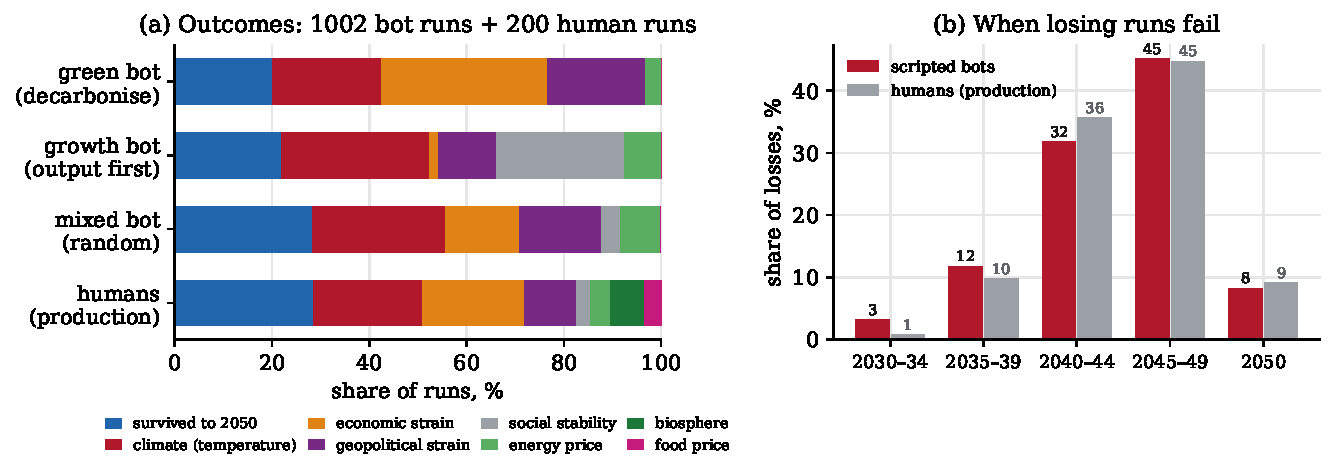
\includegraphics[width=\linewidth]{fig10_game_outcomes.pdf}
\caption{Game-mechanical simulation (1,002 automated playthroughs, 2023--2050). (a) Outcome composition by scripted policy archetype: survival share and loss causes. No doctrinaire strategy dominates; each dies of characteristic cause. (b) Timing of failures: 77\% fail 2040--2045---slow accumulators come due.}
\label{fig:game}
\end{figure}

\section{Conclusion}

Model presented links economy, climate, natural capital, society, politics, geopolitics within single loop, filling gap between specialized single-domain models. Value for strategic planning, scenario analysis, risk management lies not in point forecasting but in coherent scenario play, alternative decisions comparison, ensemble uncertainty quantification, weak-signal detection. Economic and climate blocks empirically anchored, temporal hold-out evaluated: emissions and temperature retain positive out-of-sample skill; economic fit degrades <twofold---in-sample metrics structural. Socio-political/geopolitical blocks---distinguishing feature---validated against modest but substantive criterion: improvement over naive benchmarks. Economic loop deepened: explicit money-to-prices transmission, endogenous long-run growth (R\&D-stock \`a la Jones), tested forward-looking expectations (off by default), data-grounded military-capability index. Game-mechanical layer over same core proved more than interface: outcome distributions as stress test; no doctrinaire strategy dominates; balancing surfaced and repaired two structural degeneracies invisible to retrospective validation. Residual limitations---fast climate, damage uncertainty, conflict low predictability---stated honestly; not obstacles to applying model in outlined modes. Model is exploration tool, not substitute for domain-specific expertise or policymaker judgement; outputs most informative used comparatively (scenario vs baseline) and with other evidence.

\clearpage
\appendix
\section{Key parameters and their identification}
\label{app:params}

Each parameter specified by prior distribution; central value, plausibility range (roughly the 5--95th percentile), main source. 33 key parameters have literature-grounded priors; full registry 287 parameters with calibration-status tags, most expert-set or structural; available in repository (Section~\ref{sec:repo}).

\begin{table}[h]
\centering
\small
\begin{tabularx}{\linewidth}{@{}lccL@{}}
\toprule
Parameter & Central & Range & Source \\
\midrule
Equilibrium climate sensitivity, ${}^{\circ}$C & 3.0 & 1.5--6.0 & IPCC AR6 WG1 (2021); Otto et al.\ 2013 \\
Surface heat capacity & 8.0 & 6.0--18.0 & Geoffroy et al.\ 2013 (two-layer EBM) \\
Ocean heat exchange & 1.0 & 0.4--1.3 & Geoffroy et al.\ 2013 \\
Emissions scale & 0.98 & 0.90--1.05 & Global Carbon Project 2023 \\
Structural decarbonization rate & 0.016 & 0.010--0.030 & GCP/WDI carbon-intensity trend 2000--2023; GIM 2015--2023 backtest \\
Capital share $\alpha$ & 0.30 & 0.22--0.40 & Penn World Table 10; Gollin 2002 \\
Labor share $\beta$ & 0.60 & 0.50--0.72 & Penn World Table 10; Gollin 2002 \\
Energy elasticity $\gamma$ & 0.042 & 0.015--0.080 & 2015--2023 backtest; energy literature \\
Capital--energy substitution $\sigma_{KE}$ & 0.40 & 0.20--0.60 & van der Werf 2008; Koetse et al.\ 2008 \\
Depreciation rate $\delta$ & 0.05 & 0.03--0.08 & Penn World Table 8/9 \\
TFP sensitivity to R\&D & 0.30 & 0.10--0.60 & Calibration to backtest \\
Damage coefficient & 0.0078 & 0.0015--0.025 & Howard \& Sterner 2017 (productivity-corrected central); DICE-2016R2; Burke et al.\ 2015 \\
Pure rate of time preference $\rho$ & 0.015 & 0.001--0.030 & DICE-2016R2; Stern 2007 \\
Elasticity of marginal utility $\eta$ & 1.45 & 1.0--2.0 & DICE-2016R2; Stern 2007 \\
Market demand elasticity & 0.40 & 0.20--0.70 & Labandeira et al.\ 2017 (meta-analysis) \\
\midrule
\multicolumn{4}{@{}l}{\emph{Social block (Section~\ref{sec:uq})}}\\
Tension stress from unemployment & 0.010 & 0.007--0.014 & Di Tella et al.\ 2001 (misery-index evidence); structural prior \\
Tension stress from inflation & 0.005 & 0.003--0.007 & Di Tella et al.\ 2001 (unemployment:inflation aversion $\approx$2:1); prior \\
Inequality effect on tension & 0.0005 & 0.0003--0.0007 & Wilkinson \& Pickett 2009 (inequality and social stress) \\
Trust-anchor strength & 0.060 & 0.039--0.081 & Calibrated to WGI trust persistence; prior\\
\bottomrule
\end{tabularx}
\end{table}

\clearpage
\section{Integration benchmark: where sectoral models stop}
\label{app:benchmark}

Breadth-of-coupling claim (Table~\ref{tab:compare}) made computational. Design literature-anchored: for three shocks, take published conclusion from named sectoral model, feed GIM same exogenous shock, ask whether GIM (a) reproduces sectoral first-order effect and (b) surfaces cross-sector consequence sectoral model cannot represent. Unit: decision-relevant conclusion, not headline number. Runs deterministic (57-country world, 10-year horizon, extreme events off); each scenario reports dose--response sweep where sectoral model's slope is zero. Harness and figures reproducible from repository (Section~\ref{sec:repo}).

Two methodological points: GIM's aggregate resource-price subsystem saturates within one simulated year; each shock injected at first cross-sector transmission variable (consumer-price wedge for carbon tax, import-bill/reserve burden for oil shock, food-supply gap for crop shock). Three spillovers differ in magnitude and shape; reported as such.

\subsection{Carbon tax (anchor: DICE)}

DICE-2016R \citep{nordhaus2017}: welfare-optimal carbon price (${\approx}\$31$/tCO$_2$ in 2015), first-order effect lower emissions; no labour market/ political economy. Fed same \$50/tCO$_2$ tax, GIM reproduces emissions decline (${\approx}5.5\%$ over 10 years) and, additionally, raises social tension, lowers trust as pass-through to energy prices feeds inflation/ unemployment---political-economy channel behind reversals (French 2018, Australian 2014). Tension response rises monotonically with rate (Fig.~\ref{fig:bench-carbon}); DICE response on that axis zero.

\begin{figure}[t]
\centering
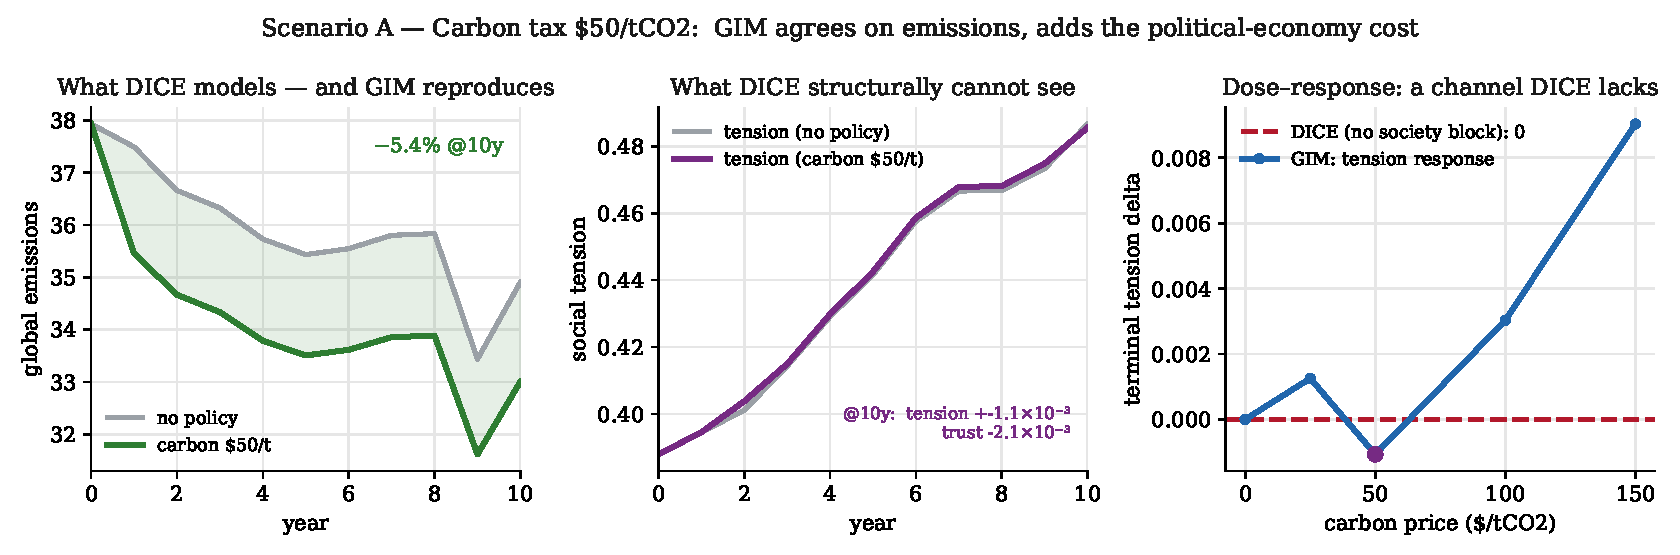
\includegraphics[width=\linewidth]{fig6_integration_carbon.pdf}
\caption{Carbon-tax scenario. Left: GIM reproduces emissions decline DICE models. Middle: GIM adds social-tension response DICE cannot represent. Right: tension response to tax rate has non-zero GIM slope vs DICE zero.}
\label{fig:bench-carbon}
\end{figure}

\subsection{Oil price shock (anchor: energy-system models)}

Energy-system model (MESSAGEix) resolves oil-supply shock as price rise/demand adjustment, bounded in energy sector. GIM carries further into sovereign finance: higher import bill, financed by reserves/debt, brings fiscally fragile importers to debt-crisis thresholds. Realistic shock (20\% supply cut, ${\approx}3\%$ GDP burden): marginal---two additional importers enter crisis. Severe shock (${\approx}15\%$ GDP burden, comparable to the worst historical episodes): mean importer debt-crisis exposure rises ${\approx}3{\times}$; four further countries enter sovereign crisis (Fig.~\ref{fig:bench-oil}). Response threshold-stepped; energy-system model produces no sovereign crises. Mechanism behind Sri Lanka 2022 default.

\begin{figure}[t]
\centering
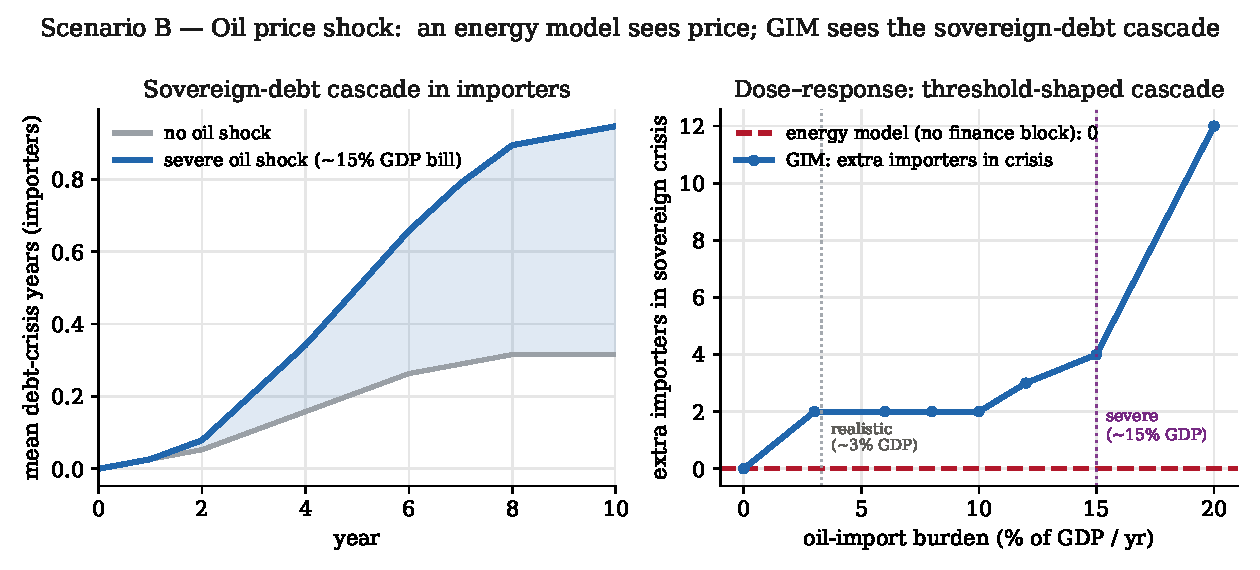
\includegraphics[width=\linewidth]{fig7_integration_oil.pdf}
\caption{Oil-price-shock scenario. Left: importer sovereign-debt-crisis duration under severe shock. Right: response to import burden threshold-stepped, marking marginal vs severe points against energy-system zero.}
\label{fig:bench-oil}
\end{figure}

\subsection{Crop yield shock (anchor: AgMIP and AR6)}

Crop assessments (AgMIP, IPCC AR6) stop at yield decline, food-security index. GIM carries yield loss further into domestic instability: cutting production/reserves of income-vulnerable importers opens food-supply gap raising protest pressure; escalation accelerates with loss depth. Nonlinear "crossing into high impact" for food prices and Arab Spring \citep{lagi2011food} (threshold FAO index 210). At severe 50\% regional yield loss, food-affordability stress rises ${\approx}0.11$, protest pressure ${\approx}0.016$ on vulnerable subset (Fig.~\ref{fig:bench-crop}); further chain attenuates toward regime fragility; endpoint domestic instability, not interstate conflict.

\begin{figure}[t]
\centering
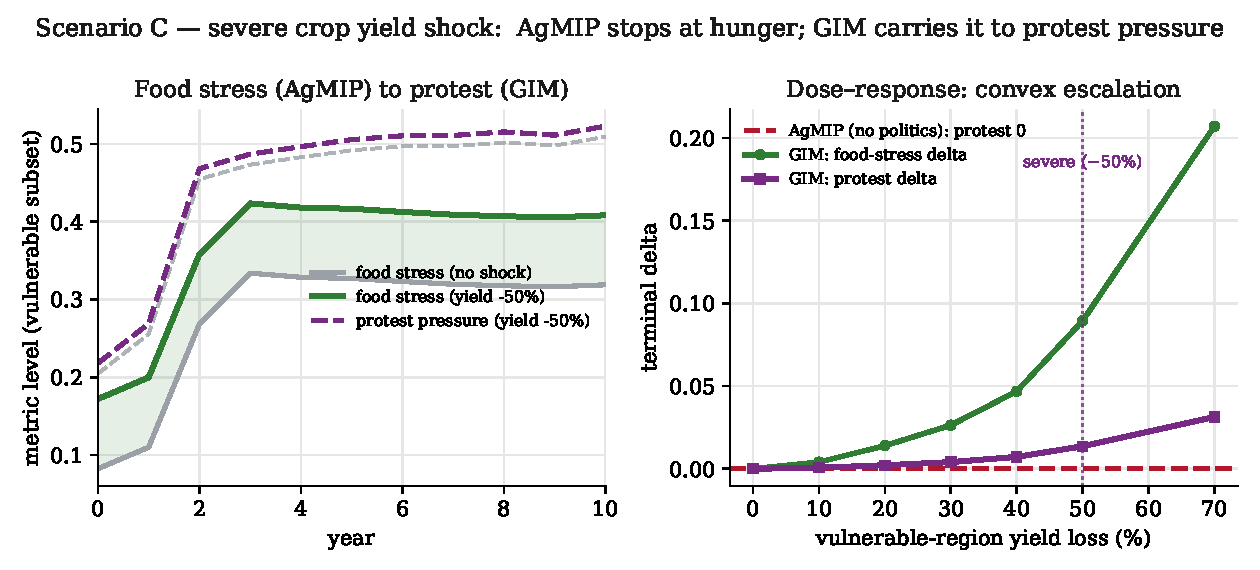
\includegraphics[width=\linewidth]{fig8_integration_crop.pdf}
\caption{Crop-yield-shock scenario. Left: food-affordability stress and protest pressure on vulnerable subset. Right: response to yield-loss depth convex against AgMIP zero on protest axis.}
\label{fig:bench-crop}
\end{figure}

Across three channels (Fig.~\ref{fig:bench-summary}) GIM exhibits positive measurable slope on axis where every sectoral model flat at zero. That gap---not single number---is integration dividend, exactly dimension coverage table summarizes qualitatively.

\begin{figure}[t]
\centering
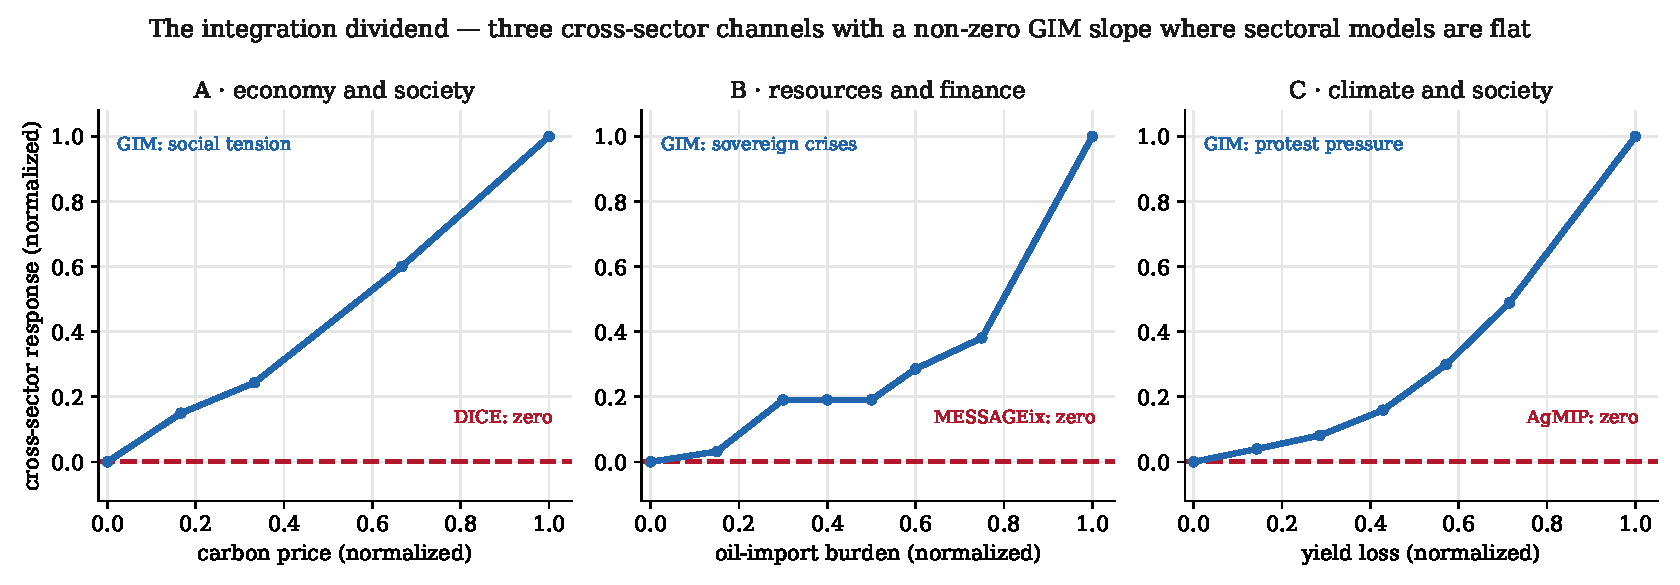
\includegraphics[width=\linewidth]{fig9_integration_summary.pdf}
\caption{Integration dividend. Each panel cross-sector channel, normalized to own maximum; dashed line every sectoral model's zero response. GIM slope smooth (economy-society), threshold-stepped (resources-finance), convex (climate-society).}
\label{fig:bench-summary}
\end{figure}

\clearpage
\bibliographystyle{plainnat}
\bibliography{references}

\end{document}